\section{Multi-Domain Multimodal Time-Series Dataset: \model}
We first introduce the key challenges in constructing \model, followed by the construction pipeline. We then detail each component of the pipeline with corresponding data quality verification. Finally, we discuss considerations for fairness and data release.


\par \noindent \textbf{Challenges.} Creating a high-quality, multi-domain numerical-text series dataset presents significant challenges, encompassing the effective gathering, filtering, and alignment of useful textual data. First, \underline{textual sources are sparse}. Unlike numerical data, typically provided by a "packaged" source, textual data are collected from a variety of dispersed sources, such as reports and news articles, necessitating extensive individual collection efforts. Second, \underline{textual information is noisy}. Raw textual data often contains large portions of irrelevant information and potential data contamination, such as expert predictions in reports, requiring rigorous filtering processes to ensure data quality. Third, \underline{textual data requires precise alignment}. It is essential to achieve temporal alignment between textual and numerical data by synchronizing reported times with numerical time steps (e.g., the time step where text is posted) and ensuring that the effective duration of textual information matches the relevant time frames at various granularities (e.g., a seasonal report should correspond to 12 time steps in a weekly time series). Additionally, the dataset faces challenges regarding ease of use, maintenance, and regular updates to remain relevant and useful for ongoing research and applications.

\begin{figure}[t]
    \centering
    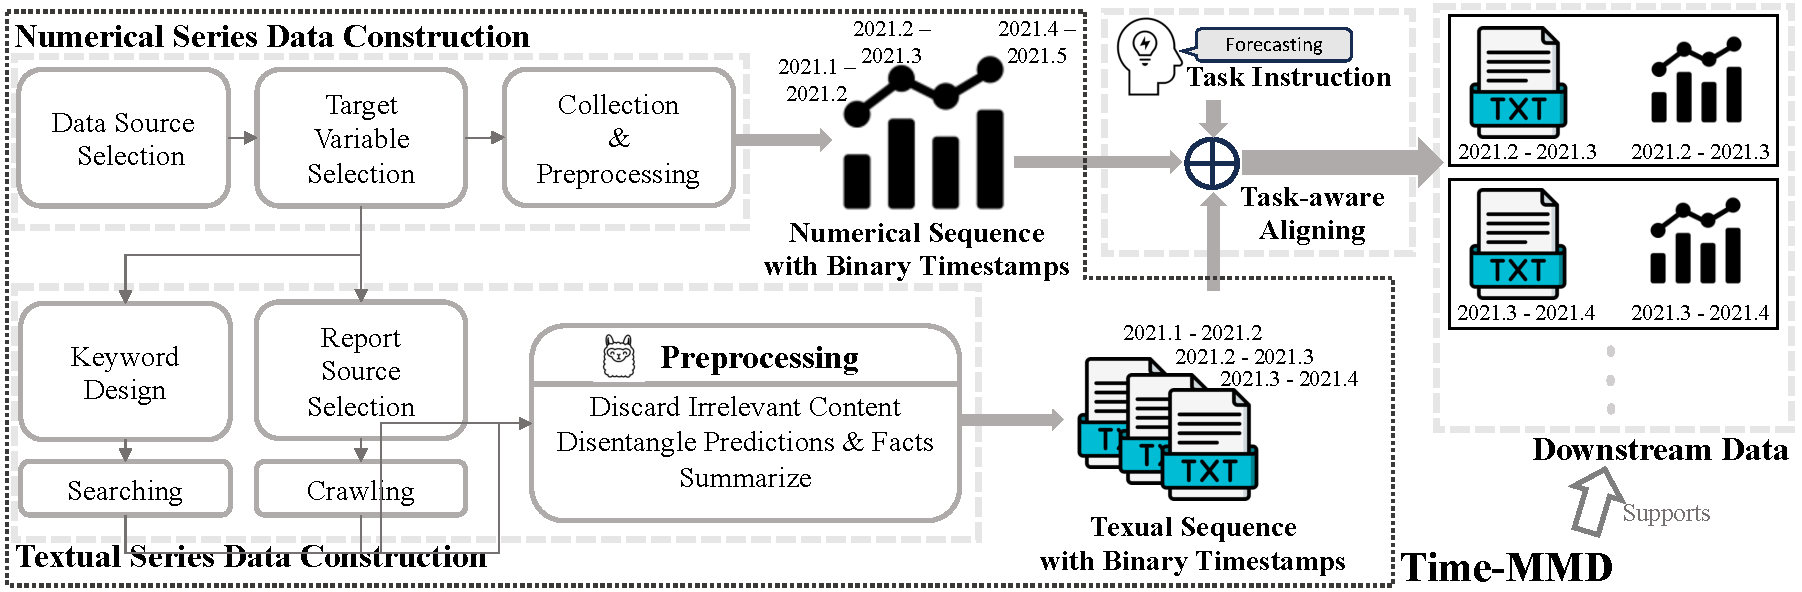
\includegraphics[width = \linewidth]{Figures/model_overview.pdf}
    \caption{Overview of the \model construction. We first construct numerical data, then construct textual data from search and report sources with LLM preprocessing targeted at the numerical data, and finally annotate the data with binary timestamps to support various downstream tasks.}
    \label{fig:overview}
\end{figure}

\par \noindent \textbf{Pipeline Overview.} We propose a comprehensive pipeline for constructing a text-numeric series dataset utilizing modern LLMs. As illustrated in Figure \ref{fig:overview}, the construction process is divided into three key steps: (1) \underline{Numerical Series Data Construction.} We gather numerical data from reputable sources to ensure reliability and accuracy. (2) \underline{Textual Series Data Construction.} Textual data is collected for fine-grained matching with the numerical data. The quality of this matching is ensured through human selection of data sources and raw text filtering by LLMs. Additionally, LLMs are employed to disentangle facts and predictions and generate summaries. (3) \underline{Numerical-Textual Alignment.} We use binary timestamps to mark the start and end dates as a universal temporal alignment method between numerical and textual series, supporting the requirements of various downstream TSA tasks.



\subsection{Numerical Series Data Construction}
\par \noindent \textbf{Data Source Selection.} We select data sources that are (1) reliable, containing verified knowledge; (2) actively released, allowing for updates with new data; and (3) multi-domain, covering various TSA patterns. Appendix~\ref{app:domain} provides considerations for domain selection. Based on these principles, we choose nine data sources from different domains, as shown in Appendix~\ref{app:data source}. Most sources are from government agencies, with the lowest update frequency being six months. 

\par \noindent \textbf{Target Variable Selection.} For each domain, we select target variables with significant real-world implications, indicating easier text matching, as shown in Table~\ref{tab:series}. These variables span three distinct frequencies: daily, weekly, and monthly. 

\par \noindent \textbf{Collection \& Preprocessing.} We collect raw data for all available times, either from batch-released files or through individual scraping. We preprocess the data by discarding early years with a high proportion of missing values. We maintain the original frequency for most domains, adjusting it for security and climate domains due to irregular releases and difficult text matching, respectively. Figure \ref{fig:OT_visualize} illustrates the diverse patterns present in each domain, such as periodicity and trends.

\par \noindent \textit{\underline{Data Quality \& Property.}} As shown in Table~\ref{tab:series} and Figure \ref{fig:OT_visualize}, the constructed numerical data provides comprehensive temporal coverage, ranging from the earliest in 1950 to the present, and exhibits distinct patterns, such as periodicity and trends.



\begin{table}[]
\centering
\caption{Overview of numerical data in \model, covering key variables across nine domains with daily, weekly, or monthly frequencies, sourced from reputable government departments. Eight domains are updated to May 2024; the environment domain update is scheduled for June 2024. We focus on univariate time series forecasting for the target variable, as \model requires constructing aligned textual data. Covariates are provided for some datasets to inspire future research which are revealed in the dimension column. \label{tab:series}}
\resizebox{\textwidth}{!}{
% \begin{tabular}{lllll}

\begin{tabular}{cccccc}
\toprule
Domain & Target &Dimension & Frequency & Number of Samples & Timespan \\ \midrule
Agriculture & Retail Broiler Composite  &1  & Monthly & $496$ & 1983 - Present \\
Climate  & Drought Level &5 & Monthly & $496$ & 1983 - Present \\
Economy & International Trade Balance &3 & Monthly & $423$ & 1989 - Present \\
Energy & Gasoline Prices &9 & Weekly & $1479$ & 1996 - Present \\
Environment & Air Quality Index&4 & Daily & $11102$ & 1982 - 2023 \\
Health & Influenza Patients Proportion &11 & Weekly & $1389$ & 1997 - Present \\
Security & Disaster and Emergency Grants &1& Monthly & $297$ & 1999 - Present \\
Social Good & Unemployment Rate &1 & Monthly & $900$ & 1950 - Present \\ 
Traffic & Travel Volume &1& Monthly & $531$ &1980 - Present \\ \bottomrule
\end{tabular}
}

\end{table}
\begin{figure}
    \centering
    \subfloat[Agriculture]{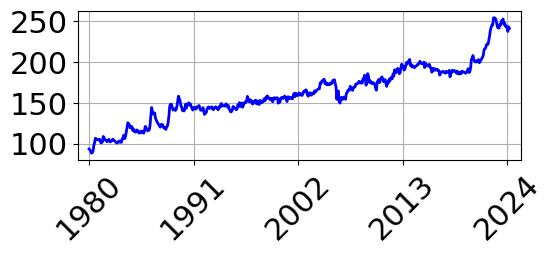
\includegraphics[height=0.094 \linewidth]{Figures/OT_Agriculture.png}}
    \subfloat[Climate]{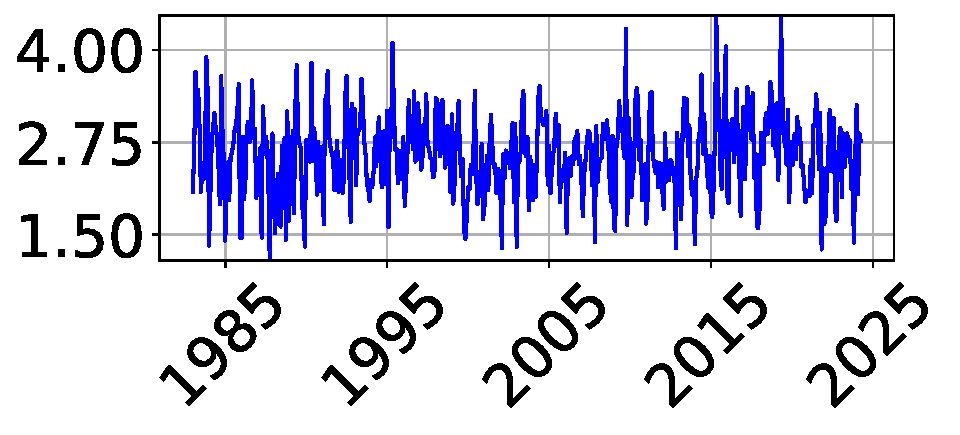
\includegraphics[height=0.09 \linewidth]{Figures/OT_Climate.pdf}}
    \subfloat[Economy]{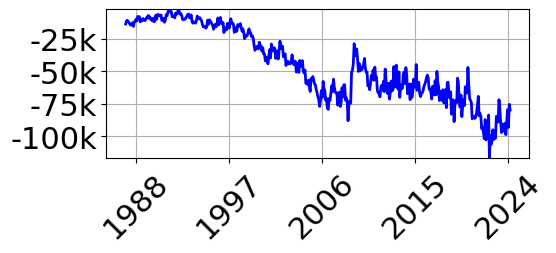
\includegraphics[height=0.09 \linewidth]{Figures/OT_Economy.png}}
    \subfloat[Energy]{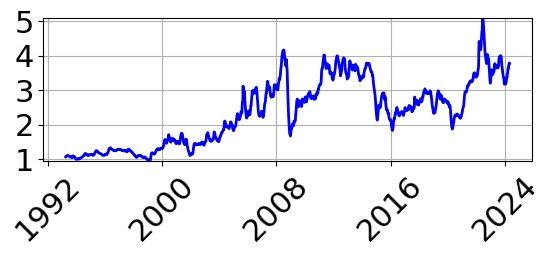
\includegraphics[height=0.094 \linewidth]{Figures/OT_Energy.png}}
    \subfloat[Environment]{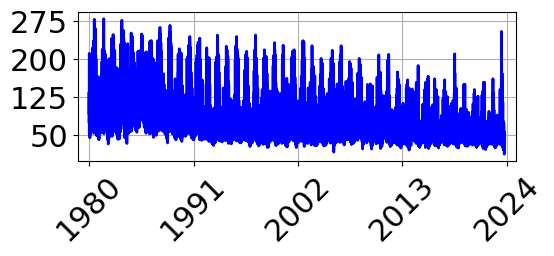
\includegraphics[height=0.091 \linewidth]{Figures/OT_Environment.png}}
    \\
    \subfloat[Health(US)]{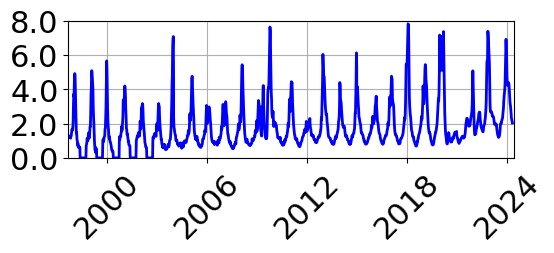
\includegraphics[height=0.092 \linewidth]{Figures/OT_Health.png}}
    \subfloat[Health(AFR)]{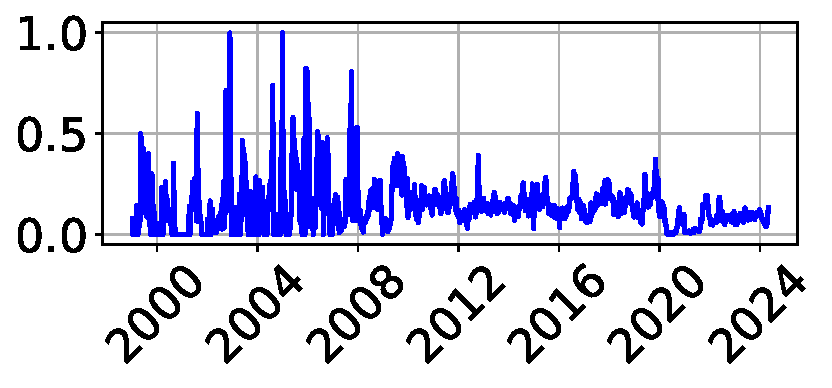
\includegraphics[height=0.09 \linewidth]{Figures/OT_AFRHealth.pdf}}
    \subfloat[Security]{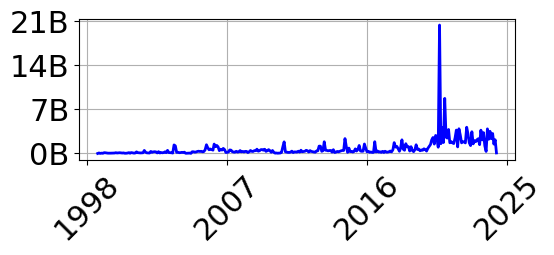
\includegraphics[height=0.09 \linewidth]{Figures/OT_Security.png}}
    \subfloat[Social Good]{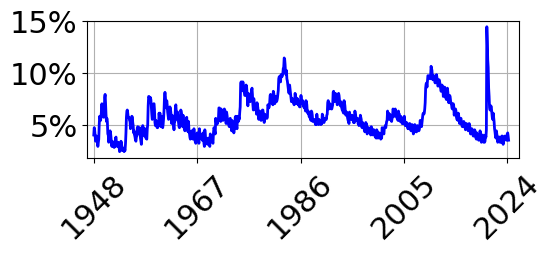
\includegraphics[height=0.09 \linewidth]{Figures/OT_SocialGood.png}}
    \subfloat[Traffic]{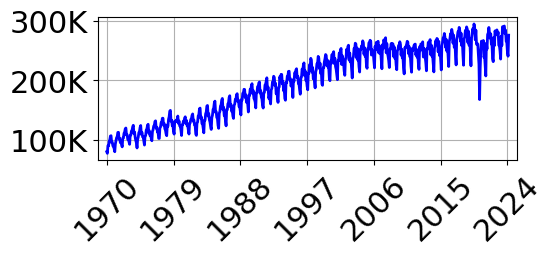
\includegraphics[height=0.09 \linewidth]{Figures/OT_Traffic.png}}
    
    \caption{Visualization of \model, highlighting distinct characteristics across different domains.}
    \label{fig:OT_visualize}
\end{figure}
% tell absent values (like earlier series are skipped); wait for unsure data source
\subsection{Textual Series Data Construction}\label{sec_text_construct}
\par \noindent \textbf{Data Source Selection: Selected Reports and Web Search Results.}
The choice of data sources should take into account both extensive coverage and initial strong relevance to the numerical data. Consequently, we combine two appropriate data source types as follows: (1) Selected Reports: For each target variable, we manually select 1-2 highly relevant report series with guaranteed updates. For instance, the weekly influenza report\footnote{https://www.cdc.gov/flu/weekly/weeklyarchives2023-2024/week04.htm} published by the Centers for Disease Control and Prevention of the United States is chosen as one of the report sources for the weekly influenza patients proportion of the United States. (2) Web Search Results: For each target variable, we design 2-3 highly relevant keywords used for web searching. 

These two data sources complement each other: report data ensures higher relevance but cannot guarantee all-time coverage, while search results cover all times but are highly redundant; search results aggregate multiple data sources, while report data, usually in PDF or TXT format, cannot be extracted by searching. For frequency alignment, the textual data covers multiple frequencies, with search texts enabling daily precision and reports ranging from weekly to monthly and yearly intervals. Appendix~\ref{app:data source} provides a complete list of keywords and reports source.

\par \noindent \textbf{Data Collection: Searching and Crawling.} For keyword web searching, we use the official Google API\footnote{https://developers.google.com/custom-search/v1/overview} as the entry point. For each keyword, we collect the timestamp, source, title, and content from the top 10 results located each week from 1980 to present. For report data, we parse all available reports from each data source and preserve only plain-text paragraphs.

\par \noindent \textbf{Data Preprocessing: Filtering, Disentangling, and Summarizing.}
To curate the collected raw text data, we introduce three key preprocessing steps: (1) Filtering to improve relevance; (2) Disentangling facts with predictions to mitigate data contamination; (3) Summarizing for better usability. Given the impracticality of performing these steps manually, we leverage the state-of-the-art LLM, Llama3-70B, to accomplish these tasks.

The prompt used for LLMs is detailed in Appendix \ref{app:prompt}. We incorporate three specific strategies to alleviate the hallucination issue in LLMs and enhance preprocessing quality: (1) A concise introduction of the text. (2) Mandating the LLM to reference the data source, aiding constraint and verification. (3) Permitting the LLM to indicate `not available' when relevance is uncertain, to avoid fabrication. Appendix \ref{app:showcase} provides a showcase of the text before and after processing.

\par \noindent \textit{\underline{Data Quality \& Property.}} Overall, Figure~\ref{fig:factPerMonth} visualizes the extracted fact count per month over time by domain. Note that the Agriculture report data is of high volume around 2020 and therefore produces a peak. We make the following observations: (a) The search data count exhibits a gradual increasing trend, benefiting from the development of the Internet; the report data count has stabilized in recent years, indicating that release schedule has become stable. (b) The sparsity of textual data varies across different domains, with high-profile fields often accompanied by richer textual data. These validate the extensibility and updatability of \model and highlight the importance of its coverage across 9 diverse domains. 

We further validate the effectiveness of key steps in textual data construction:

(a) Data sources selection. We use \textit{relevance} and \textit{coverage} ratio to describe the percentage of relevant texts and the proportion of numerical series data being covered by at least one fact, respectively. As demonstrated by Table~\ref{tab:LLMPre}, report data exhibits higher relevance but lower coverage; search data display the opposite pattern. Thus, our combined usage serves as a comprehensive solution.

(b) Data preprocessing. Figure~\ref{fig:wordcloud} provides word cloud visualizations of constructed text data in the health domain, respectively for extracted facts, extracted predictions, and discarded text. Recall that the target variable here is the influenza patients proportion.  Highly relevant words such as "pandemic", "vaccine", and "flu" appear more frequently in the extracted facts; research paper-related words such as "edu", "mdpi", and "university" are more common in the discarded text. Besides, the prediction text primarily contains words describing future, such as "will" and "next". These validate the effectiveness of LLM filtering and disentangling. Furthermore, Table~\ref{tab:LLMPre} presents a comparison of the token count before and after preprocessing. The substantial decrease validates that LLM summarizing improves usability. Appendix~\ref{app:manual} provides the manual verification results on a subset of the data to further validate the effectiveness of preprocessing using LLMs.

\begin{table}[]
\centering
\caption{Statistics for text data. Relevance indicates the percentage of text data with relevant content. Coverage describes the proportion of numerical series data being covered by at least one fact. Details are provided in Appendix \ref{app:text_statistics}. The statistics highlight the need for both reports and search data.}
\resizebox{\textwidth}{!}{
\begin{tabular}{@{\extracolsep{4pt}}cccccccc}
\toprule
\multicolumn{1}{c}{\multirow{2}{*}{Source}} & \multirow{2}{*}{\begin{tabular}[c]{@{}c@{}}Raw\\ Tokens\end{tabular}} & \multicolumn{3}{c}{Preprocessed Extracted Facts} & \multicolumn{3}{c}{Preprocessed Extracted Prediction} \\ \cline{3-5} \cline{6-8}
\multicolumn{1}{c}{} & & Relevance(\%) & Coverage (\%) & Tokens &Relevance(\%) & Coverage (\%)  & Tokens \\ \midrule
Report & $17.4$k & $84.3${\tiny $\pm 27.2$} & $34.1${\tiny $\pm 26.8$} & $37.6${\tiny $\pm11.9$} & $82.3${\tiny$\pm28.5$} & $33.8${\tiny $\pm27.3$} & $74.6${\tiny $\pm16.1$} \\
Search & $54.4$ & $16.8${\tiny $\pm 3.3$} & $90.7${\tiny $\pm 13.5$} & $38.4${\tiny $\pm 4.0$} & $16.0${\tiny $\pm4.3$} & $81.9${\tiny $\pm17.2$} & $62.8$ {\tiny $\pm 3.3$}\\ 
\bottomrule
\end{tabular}
}

\label{tab:LLMPre}
\end{table}


\begin{figure}
    \centering
    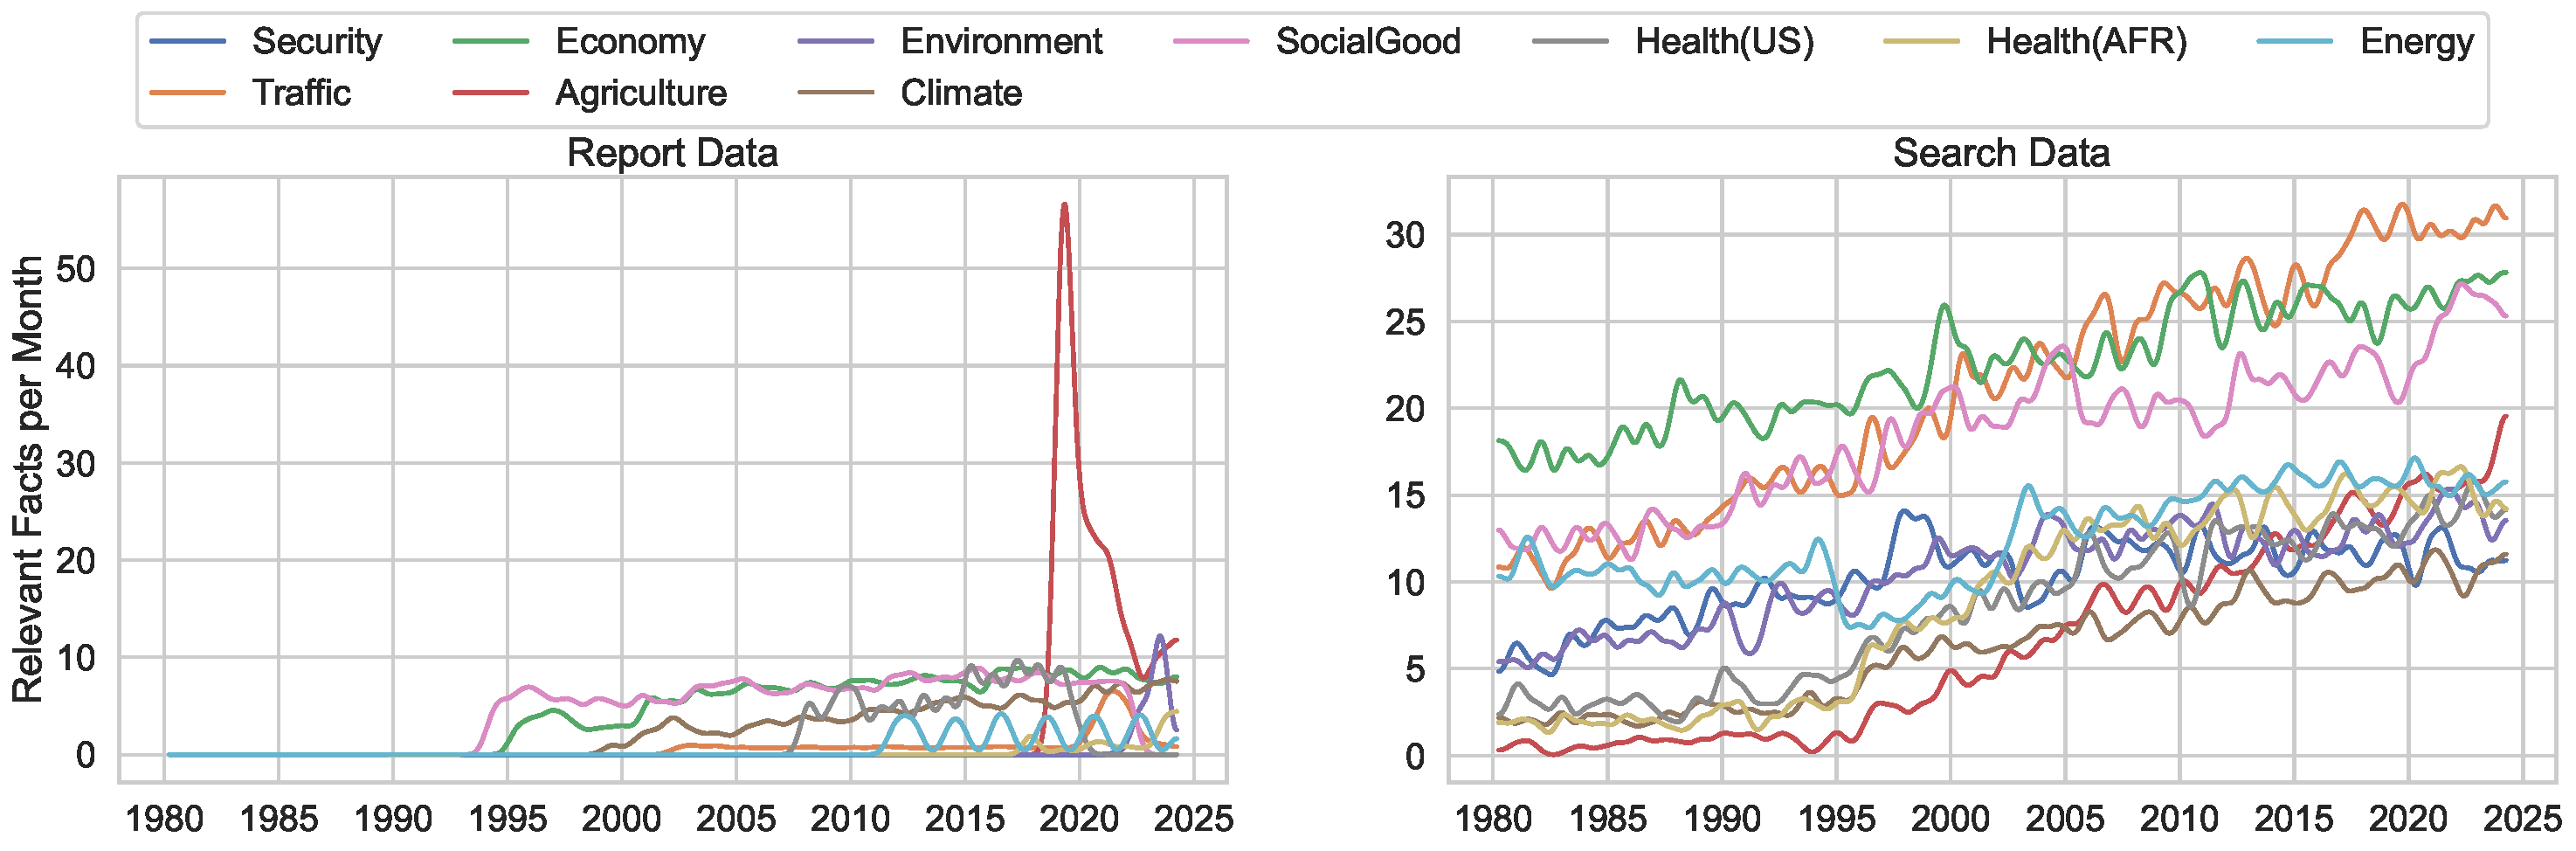
\includegraphics[width = \linewidth]{Figures/moving_cov.pdf}
    \caption{Visualization of relevant report (a, left) and search (b, right) counts in \model over time. Text counts from both reports and searches increase over time. Domains receiving more attention, such as the economy, contain more available relevant text data..}
    \label{fig:factPerMonth}
\end{figure}

\begin{figure}
    \centering
    \subfloat[Word cloud visualization for extracted facts]{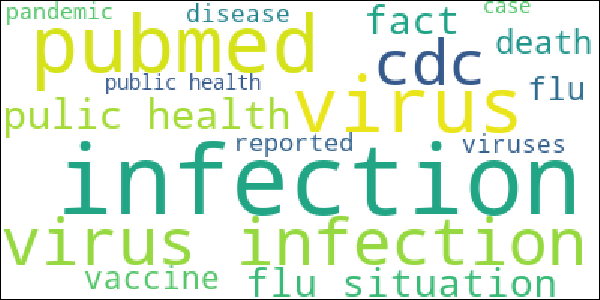
\includegraphics[width = 0.32 \linewidth]{Figures/wordcloud_health_search_fact.pdf}}
    \hfill
    \subfloat[Word cloud visualization for extracted predictions]
    {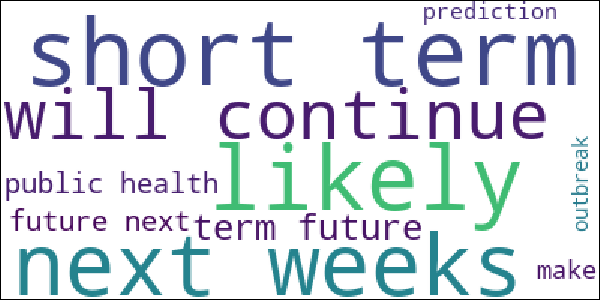
\includegraphics[width = 0.32 \linewidth]{Figures/wordcloud_health_search_pred.pdf}}
    \hfill
    \subfloat[Word cloud visualization for extracted discarded text]{
\includegraphics[width=0.32\linewidth]{Figures/wordcloud_health_search_discarded.pdf}}
    \caption{Word cloud visualization for influenza patient proportion from the health domain. The discarded texts are identified by the LLM as irrelevant to the target variable. The results validate the effectiveness of LLM preprocessing.}
    \label{fig:wordcloud}
\end{figure}


\subsection{Binary Time Stamps for Diverse TSA Tasks}
To enable the \model for versatile and flexible use, we maintain binary timestamps for all numerical and text data, storing the manually verified start dates and end dates. Such binary stamps can be easily referred to while serving different tasks. For report text data, we manually verify the timestamps based on the release notes or report contents. For search data, we integrate adjacent search results within each week and mark timestamps correspondingly.
\subsection{Considerations for Fairness and Data Release}
To consider fairness, we gather data from both the United States and African regions in the Health domain. As depicted in Figure~\ref{fig:OT_visualize}, the numerical data of African region exhibits weaker periodicity. Figure~\ref{fig:factPerMonth} shows that the African region has considerably fewer reports compared to the United States. We encourage researchers to consider underrepresented groups when conducting multimodal TSA tasks.

To support various existing and potential novel TSA tasks, we include the following metadata when releasing \model: (1) Numerical Data: start \& end time, target variable, other variables; (2) Text Data: start \& end time, fact text (content \& data source), prediction text (content \& data source).
